
\section{イントロダクション}
卒業論文は,大学で課される普通の授業のレポートに比べて多くの情報内容が要求されます.また,研究という側面から体裁や版権など多くの出版における掟を遵守しながら,高い品質を保つ必要です.そのため,指導教官との編集作業が重要となるます.編集作業の効率を高めるためには,共同作業を促進するプラットフォームが必要です.

体裁などを考えるとLatexの使用が標準ですが,執筆段階での煩わしさを低減するため,Mark Up記法による文章作成が一般的です(「ドキュメント作成システム構築ガイド,GitHub, RedPen, Asciidoctor, CIによるモダンライティング」, 伊藤敬彦,吉村孝広,技術評論社).西谷研ではMark Up記法の一種であるhiki記法を用いて執筆します.hiki記法からhtmlへ変換するソフトhikidocによる容易な変換が可能なため,日記web appliのhiki diaryでも利用されている有名なソフトです.hiki記法をベースにして,wiki wiki webと同等の機能を提供するhikiシステムがgithubに公開されており,個人の手持ちのパソコンにインストールしてwikiを利用することができます.西谷研ではさらにhiki記法を拡張して,コードのカラー表示,数式のlatex記述が可能となるシステムを利用しています.

本資料では,卒論の編集作業を効率化する図に示すようなシステムの使い方を紹介します.

\begin{figure}[htbp]\begin{center}
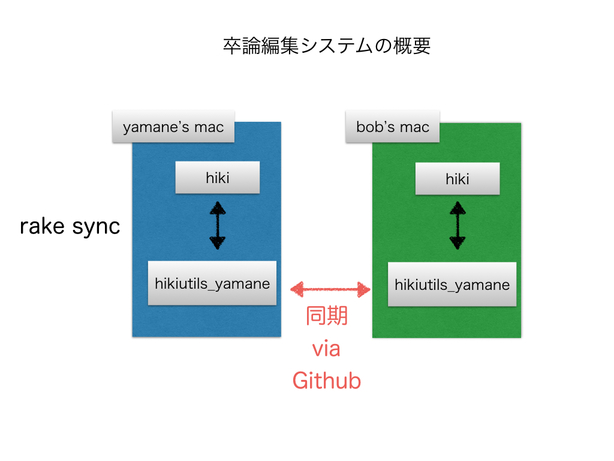
\includegraphics[width=6cm,bb=0 0 442 500]{../figs/./hikiutils_bob.002.jpeg}
\caption{卒論編集システムの概要.}
\label{default}\end{center}\end{figure}
例えば,卒業生をyamaneとしましょう.yamaneの個人のMacの自分のdirectory(hikiutils\_yamane)に幾つかのファイルを作成して卒論を書いているとします.これを指導教官(bob)が編集するとします.この同期には,Githubにより提供される共同作業環境を使います.これだけでは編集中の文書の体裁がわかりにくいでしょう.そこで,hikiシステムにより容易にwebブラウザ上に完成形を表示しつつ執筆することが求められます.このような操作環境を提供するのが,hikiutils -iです.

\section{hikiとの同期}
\subsection{hikiutilsのinstall}
hikiuitlsをgemからinstallしておく必要がある.コマンドは以下の通り.
\begin{quote}\begin{verbatim}
gem install hikiutils
\end{verbatim}\end{quote}
さらに
\begin{quote}\begin{verbatim}
hiki -v
\end{verbatim}\end{quote}
で0.2.3.2以上であることを確認.

\subsection{個別ディレクトリーの構成}
図にhikiutils\_bobのディレクトリー構成を示す.

\begin{figure}[htbp]\begin{center}
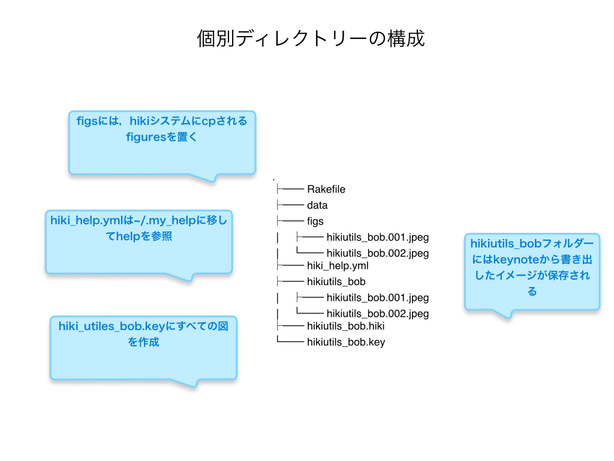
\includegraphics[width=6cm,bb=0 0 442 500]{../figs/./hikiutils_bob.003.jpeg}
\caption{hikiutils\_bobのディレクトリー構成.}
\label{default}\end{center}\end{figure}
コマンド
\begin{quote}\begin{verbatim}
hiki -i
\end{verbatim}\end{quote}
によって以下のようなファイルが作成される.
\begin{lstlisting}[style=]
bob% ls -lat
total 1072
-rw-r--r--   1 bob  501      99  1 20 12:44 .hikirc
drwxr-xr-x   5 bob  501     170  1 20 12:44 figs/
drwxr-xr-x  12 bob  501     408  1 20 12:34 ./
-rw-r--r--   1 bob  501       8  1 20 11:01 .gitignore
-rw-r--r--   1 bob  501    3507  1 20 11:01 Rakefile
drwxr-xr-x   2 bob  501      68  1 20 11:01 data/
-rw-r--r--   1 bob  501    2595  1 20 11:01 hiki_help.yml
drwxr-xr-x  26 bob  501     884  1 20 11:00 ../
\end{lstlisting}
この.hikircにデータが設定データが自動的に入る.さらにhikiutils\_bob.hikiおよびhikiutils\_bob.keyを作成する.これで執筆ファイルの基本構成が出来上がる.

keynoteで図を作成して,hikiutils\_bob.hikiに文章を記述していく.

\subsection{一般的な執筆手順}
\begin{enumerate}
\item 書類の作成
\begin{enumerate}
\item open -a mi hikiutils\_bob.hiki
\end{enumerate}
\item keynoteを開ける
\begin{enumerate}
\item open hikiutils\_bob.key
\end{enumerate}
\item keynoteのイメージをfigsに
\begin{enumerate}
\item keynoteでイメージへ書き出し(hikiutils\_bobを仮定)
\item rake convert 80 hikiutils\_bob
\end{enumerate}
\item hikiシステムとの同期
\begin{enumerate}
\item rake sync
\end{enumerate}
\item hikiシステムで表示
\begin{enumerate}
\item hiki -u hikiutils\_bob
\end{enumerate}
\end{enumerate}
\subsection{rakeが用意しているタスク}
rakeの用意しているコマンドは次のとおり.
\begin{lstlisting}[style=]
rake sync             # hikiの同期
rake force_sync       # hikiの強制同期
rake chenv            # For hiki Errno::ENOENT, Errno::EACCES

rake convert          # convert fig size SCALE TARGET_DIR
rake increment        # increment fig NUBERS in FILE
rake number           # numbering figs from the NUBER in FILE

rake touch            # hikiシステムを最新状態に更新
rake github           # Githubのdirをsafariでopen
\end{lstlisting}
\subsubsection{rake sync}
hikiutils\_bobにある必要な書類をhikiシステムにコピーする.その際,名前の書き換えを行う.

\begin{table}[htbp]\begin{center}
\caption{}
\begin{tabular}{lll}
\hline
hikiutils\_bobでの名前   &hikiシステムでの名前  \\ \hline
hikiutils\_bob.hiki   &hikiutils\_bob  \\
introduction.hiki   &hikiutils\_bob\_introduction  \\
\hline
\end{tabular}
\label{default}
\end{center}\end{table}
%for inserting separate lines, use \hline, \cline{2-3} etc.

figsディレクトリー内のファイルはhiki/cache/attache/hikiutils\_bobにcpされる.従って,hiki文書中で参照するには,
\verb|{{attach_view(hogehoge.png)}}|
という記述が必要となる.

\subsubsection{rake force\_sync}
hikiシステム側で直接変更を加えると,hikiutilsがsyncした時と差ができる.これを検知して,ユーザに注意を喚起する仕組みがある(rake check\_previous).これはsyncした時に自動的に呼び出される.違いの出たfilesを修正した後に強制的に同期をとるためのコマンドとして,force\_syncが用意されている.

\subsubsection{rake chenv}
hikiシステム上でerrorが出た場合(Errno::ENOENT, Errno::EACCES)に試してほしい.errorの状況は個人の設定によってちがうため,対処法の実装は網羅されていない.うまくいかない場合は西谷にIssuesとして投げるように.

\subsubsection{rake convert VAL DIR}
keynoteが吐き出したイメージを変換するためのコマンド.ImageMagickがインストールされている必要がある.ない場合は,自分でbrewからinstallするか,\verb|https://www.imagemagick.org/script/binary-releases.php|からダウンロード.うまくいかない場合はdonkeyに聞いてみてください.
\begin{quote}\begin{verbatim}
rake convert 80 hikiutils_bob
\end{verbatim}\end{quote}
によって,DIR=hikiutils\_bobにあるpngファイルをVAL=80%に縮小してfigsにためる.

\subsubsection{rake increment}
keynoteでページを追加するとhikiでの参照(attach\_view)にずれが生じる.いまのところこれを解消する方法はなく手で修正を加える必要がある.ずれが単純な場合には,
\begin{lstlisting}[style=]
cp hikiutils_bob.hiki tmp.hiki
rake increment 2 tmp.hiki > tmp2.hiki
\end{lstlisting}
としてattach\_viewのページ番号を単純に増加させることができる.

\subsubsection{rake number}
rake incrementと同じくfigs内の通し番号が変わった時にattach\_viewの通し番号を調整するコマンド.
\begin{lstlisting}[style=]
rake number 3 hikiutils_bob.hiki > tmp.hiki
cp tmp.hiki hikiutils_bob.hiki
\end{lstlisting}
とすると
\begin{quote}\begin{verbatim}
8c8
{{attach_view(hikiutils_bob.002.jpeg)}}
---
{{attach_view(hikiutils_bob.003.jpeg)}}
21c21
{{attach_view(hikiutils_bob.003.jpeg)}}
---
{{attach_view(hikiutils_bob.004.jpeg)}}
\end{verbatim}\end{quote}
などと番号を3から順に振り替えてくれる.

\subsubsection{rake touch}
hiki touchを行って最新版に更新.

\subsubsection{rake github}
git remoteにあるoriginのgithubをsafariでopen.

\subsection{githubによる同期}
\begin{enumerate}
\item git init, forkが済んでいると仮定
\item upstream, originの確認
\begin{enumerate}
\item bob% git remote -v
\end{enumerate}
\item git push作業
\begin{enumerate}
\item git add -A
\item git commit -m 'first commit'
\item git push origin master
\end{enumerate}
\item githubでbobへpull requestをかける
\item bobの編集後,通知がくる.まつことなく作業してもok.
\item git pull作業
\begin{enumerate}
\item git pull upstream master
\end{enumerate}
\end{enumerate}
これがうまくいかん時は聞いてください.

\begin{figure}[htbp]\begin{center}
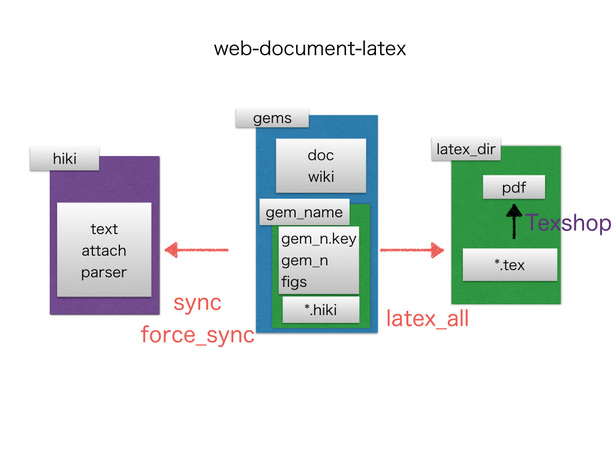
\includegraphics[width=6cm,bb=0 0 442 500]{../figs/./hikiutils_bob.004.jpeg}
\caption{卒論編集時のgithubによる同期のシーケンス図.}
\label{default}\end{center}\end{figure}
\subsection{hikiutil関連のヘルプ}
\subsubsection{hikiで卒論を書くときの初期化と掟}
\begin{itemize}
\item 開発メモ:figs,dataも作成
\item 目的:西谷が後で迷わないように決まったファイル構造を堅持すべし
\item 文書:hikiで書く.のちには,latexに変換するプログラムを提供します
\item 図表:すべての図表をkeynoteにまとめる,タイトルを分かりやすく書く
\item データ:dataディレクトリにまとめる.ファイル名をkeynoteの対応する図表中に記す
\item hiki --initializeで初期ファイル(Rakefile, ./.hikirc, hiki\_help.yml)がcopyされる
\item hiki\_help.ymlを適宜~/.my\_helpにcopyしてhiki\_helpとして利用,(my\_help参照)
\item Errno::EACCESやpermission errorがでたときはrake chenvを試してみる(報告して)
\item rake syncによってhikiディレクトリーと同期が取られる
\item hiki -u TARGETによってブラウザー表示される
\item テキストの拡張子は'.hiki'
\item hikiでのurlはテキスト前とディレクトリーから自動生成される
\item 例えば,hiki2latex\_saki/introduciton.hikiとするとhiki2latex\_saki\_introducitonと変換される
\end{itemize}
\subsubsection{error対応}
\begin{itemize}
\item Permission denied - ./data/text/boundary\_narita (Errno::EACCES)->テキストにhikiが書き込めない,chmod a+w FILE
\end{itemize}
\subsubsection{図表:すべての図表をkeynoteにまとめる,タイトルを分かりやすく書く}
\begin{itemize}
\item keynoteに書いたスライドはイメージに書き出して,rake convert 80 TARGET\_DIRでfigsに変換
\item rake syncでfigsにあるfilesはhiki/target\_dirにcpされる
\item \verb|convert #{source} -resize 20% #{target}によって,target=figs/TAERGET.pngに20%に縮小して保存される|
\item convert -density 300 view.svg view.pngで300dpiで変換
\item attach\_anchorでは
\end{itemize}
'\verb|{{attach_anchor(test.png, hiki2latex_saki)}}|'
と,directory指定しなければならない.

\begin{itemize}
\item keynoteであとで図を挿入して番号が変わった時の原稿の一括変換
\item rake increment 2 boundary\_bob.hiki boundary\_bob > tmp.hiki
\item rake convert 60 boundary\_bob
\item rake sync
\item hiki -u boundary\_bob\_tmp
\end{itemize}
